\documentclass[11pt]{article}
\usepackage[margin=1in, top=1in]{geometry}
\usepackage[all]{nowidow}
\usepackage[hyperfigures=true, hidelinks, pdfhighlight=/N]{hyperref}
\usepackage[separate-uncertainty=true, group-digits=false]{siunitx}
\usepackage{graphicx,amsmath,physics,tabto,float,amssymb,pgfplots,verbatim,tcolorbox}
\usepackage{listings,xcolor,subfig,caption,import,wrapfig,enumitem}
\usepackage[version=4]{mhchem}
\usepackage[noabbrev]{cleveref}
\newcommand{\creflastconjunction}{, and\nobreakspace}
\definecolor{stringcolor}{HTML}{C792EA}
\definecolor{codeblue}{HTML}{2162DB}
\definecolor{commentcolor}{HTML}{4A6E46}
\captionsetup{font=small, belowskip=0pt}
\lstdefinestyle{appendix}{
    basicstyle=\ttfamily\footnotesize,commentstyle=\color{commentcolor},keywordstyle=\color{codeblue},
    stringstyle=\color{stringcolor},showstringspaces=false,numbers=left,upquote=true,captionpos=t,
    abovecaptionskip=12pt,belowcaptionskip=12pt,language=Python,breaklines=true,frame=single}
\lstdefinestyle{inline}{
    basicstyle=\ttfamily\footnotesize,commentstyle=\color{commentcolor},keywordstyle=\color{codeblue},
    stringstyle=\color{stringcolor},showstringspaces=false,numbers=left,upquote=true,frame=tb,
    captionpos=b,language=Python}
\renewcommand{\lstlistingname}{Appendix}
\pgfplotsset{compat=1.17}

\begin{document}

\begin{center}
    \textbf{CP Tut 2}\hspace{2in}\textbf{KDSMIL001}\hspace{2in}\textbf{30-04-2022}
\end{center}

\begin{enumerate}
    \item Using the Lagrange interpolation method with the Regula Falsi root finding method, we were able to find the root of the function $f(x)=e^x \ln x-x^2$. \\
    To do this, we simply generated data by evaluating $y_i=f(x_i)$ for $x_i=1.0, 1.1, \dots, 2.0$ and then, choosing our starting points as the leftmost and rightmost points of the interval, used linear interpolation to find the $x$-value for which the line connecting the function evaluation at those two points crosses the $x-axis$:
    \begin{align*}
        y(x)&=y_1+\frac{(y_2-y_1)(x-x_1)}{(x_2-x_1)} \overset ! = 0\\
        \implies x&=x_1-y_1\frac{x_2-x_1}{y_2-y_1}
    \end{align*}
    This then replaced the point on the same side of the root as it and we found the function evaluation at that point by interpolation. We ran this algorithm until a tolerance was reached, in our case until the function value at the root was $|y_0|<\num{1e-5}$. 

    \begin{figure}[H]
        \begin{center}
            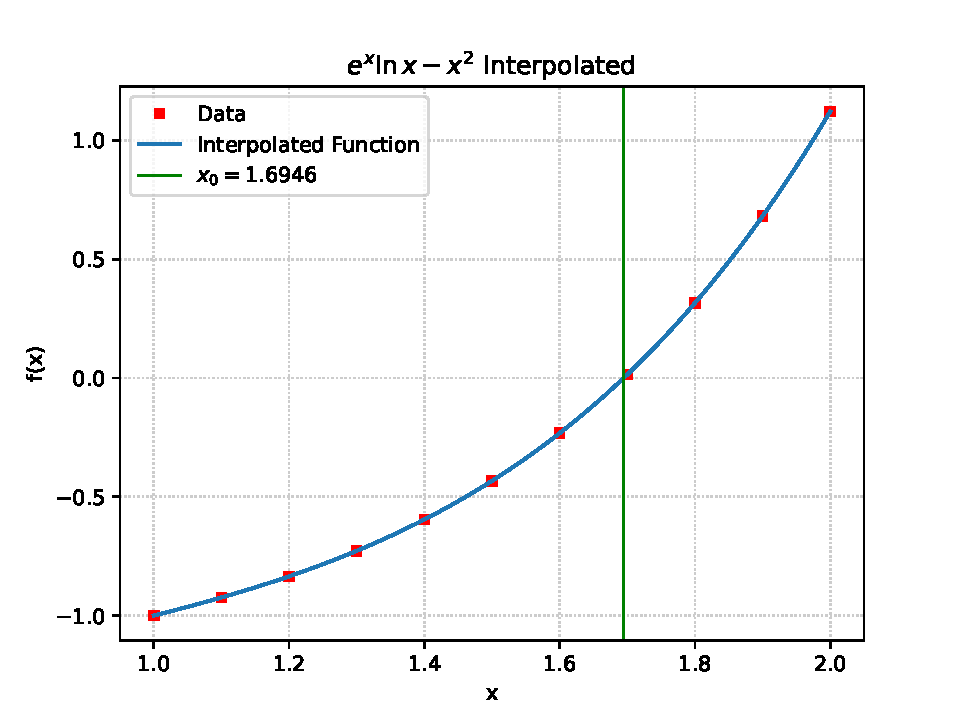
\includegraphics[width=.6\textwidth]{Plots/q1.pdf}
            \caption{Data generated from $y_i=f(x_i)=e^{x_i} \ln(x_i)-x_i^2$ with $x_i=1.0, 1.1, \dots, 2.0$, interpolated using the Lagrange interpolation method on 100 points. The root of the function $x_0$ was found using Regula Falsi and Lagrange interpolation to a tolerance of \num{1e-5}.}
            \label{fig:q1}
        \end{center}
    \end{figure}

    \item In our implementation of Smoothed Particle Interpolation, our two parameters were number of ``particles'' $N$ and smoothing length $h$. We are able to vary $N$ here, but in practice $N$ is most likely going to be fixed as the ``particles'' we choose are most likely going to be the data that we have. \\
    We began by generating our data from the function $f(x)=3x^4-3x^2$ using $N=50$ evenly spaced data points on the interval $[-10,10]$. Since SPI struggles at the boundaries of intervals, we chose to only interpolate over a smaller interval $[-5,5]$. We used the Gaussian kernel function and its derivatives
    \begin{align}
        W(x,x';h) &= \frac{1}{h\sqrt{\pi}}\exp\left(-\left(\frac{x'-x}{h}\right)^2\right) \label{eqn:GaussianKernel}\\
        W'(x,x';h) &= \frac{-2(x'-x)}{h^3\sqrt{\pi}}\exp\left(-\left(\frac{x'-x}{h}\right)^2\right) \label{eqn:GaussianKernelPrime}\\
        W''(x,x';h) &= \frac{-2}{h^3\sqrt{\pi}}\exp\left(-\left(\frac{x'-x}{h}\right)^2\right) + \frac{4(x'-x)^2}{h^5\sqrt{\pi}}\exp\left(-\left(\frac{x'-x}{h}\right)^2\right) \label{eqn:GaussianKernelPrimePrime}
    \end{align}
    where $x$ is the point at which we evaluate the function, $x'$ are the data points, which we sum over for each $x$, and $h$ is the smoothing length, i.e. the width of the Gaussian. Using these, the interpolation for the function and its first 2 derivatives was 
    \begin{align}
        f(x)&\approx \sum_i \Delta x_i f(x_i) W(x,x_i;h) \label{eqn:SPI}\\
        f'(x)&\approx -\sum_i \Delta x_i f(x_i) W'(x,x_i;h) \label{eqn:SPIPrime}\\
        f''(x)&\approx \sum_i \Delta x_i f(x_i) W''(x,x_i;h) \label{eqn:SPIPrimePrime}
    \end{align}
    where the $x_i$ are our data points, or ``particles''.\\
    With these approximations, using $N=50$ and $h=0.5$, we found were able to interpolate 1 000 points on the interval $[-5,5]$ and get the plots in \cref{fig:q2afunc}. These can be compared to the exact values of the function and its derivatives in \cref{fig:q2aexact}.
    
    What is of interest is the error between the interpolated functions and the exact value, so plotted in \cref{fig:q2a1,fig:q2a2,fig:q2a3} is the difference between the interpolated values and the exact values, for the function and its first two derivatives.
    
    We can see some rather peculiar behaviour, where the error seems to be behaving like a polynomial, such that when we differentiate the function, the error gets ``differentiated'' as well. \\

    \begin{figure}[H]
        \begin{center}
            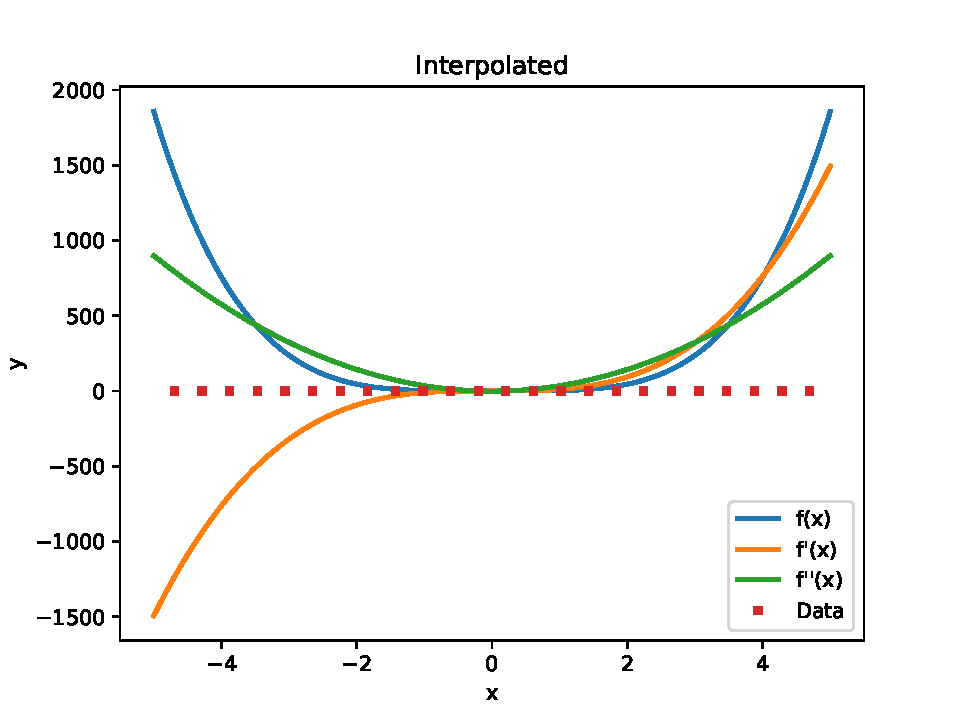
\includegraphics[width=.6\textwidth]{Plots/q2afunc.pdf}
            \caption{Data generated from $y_i=f(x_i)=3x_i^4-3x_i^2$ with $x_i\in[-10,10]$, interpolated using SPI on 1 000 points in the interval $[-5,5]$ to find the function value as well as its first two derivatives.}
            \label{fig:q2afunc}
        \end{center}
    \end{figure}
    
    \begin{figure}[H]
        \begin{center}
            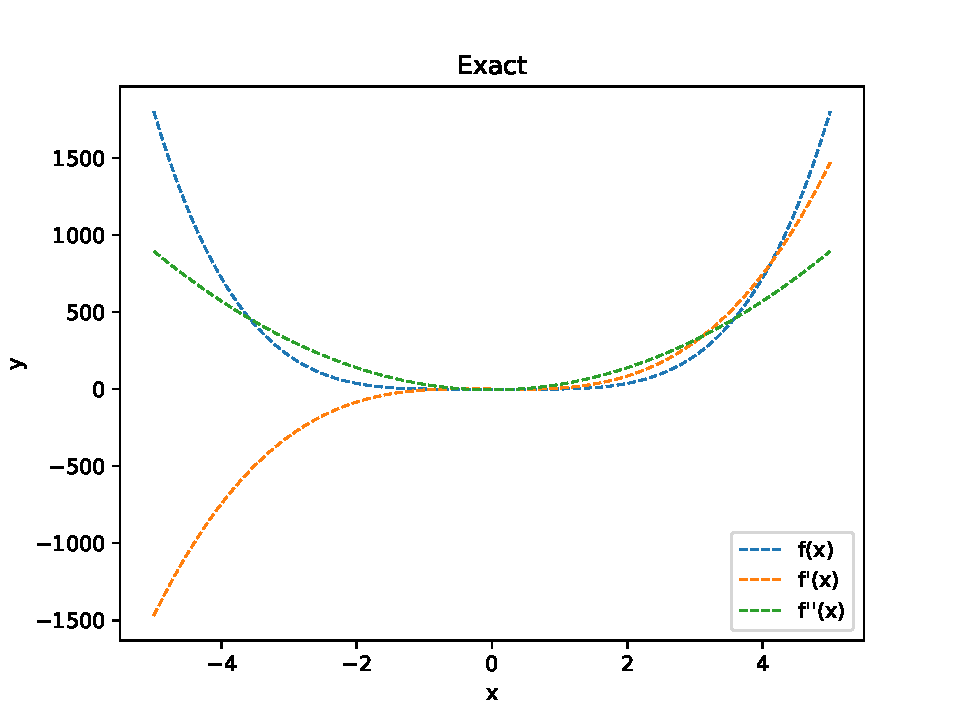
\includegraphics[width=.6\textwidth]{Plots/q2aexact.pdf}
            \caption{The exact form of the function $f(x)=3x^4-3x^2$ and its first two derivatives, evaluated on 1 000 points in the interval $[-5,5]$.}
            \label{fig:q2aexact}
        \end{center}
    \end{figure}
    
    \begin{figure}[H]
        \begin{center}
            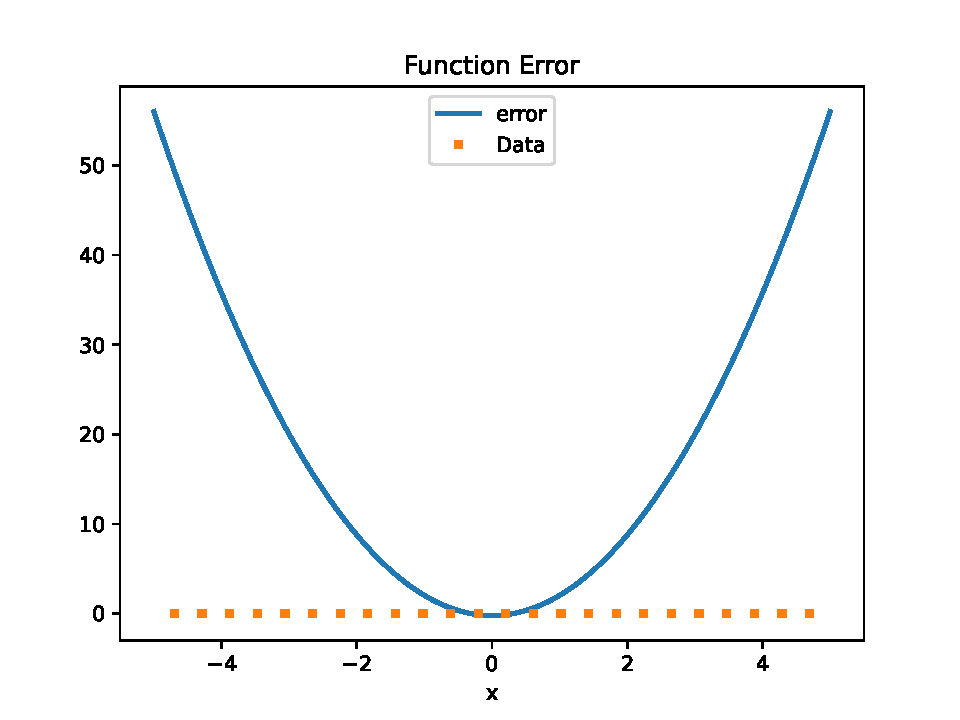
\includegraphics[width=.6\textwidth]{Plots/q2a1.pdf}
            \caption{Error between the interpolated values and the exact values for $f(x)=3x^4-3x^2$ on 1 000 points in the interval $[-5,5]$.}
            \label{fig:q2a1}
        \end{center}
    \end{figure}

    \begin{figure}[H]
        \begin{center}
            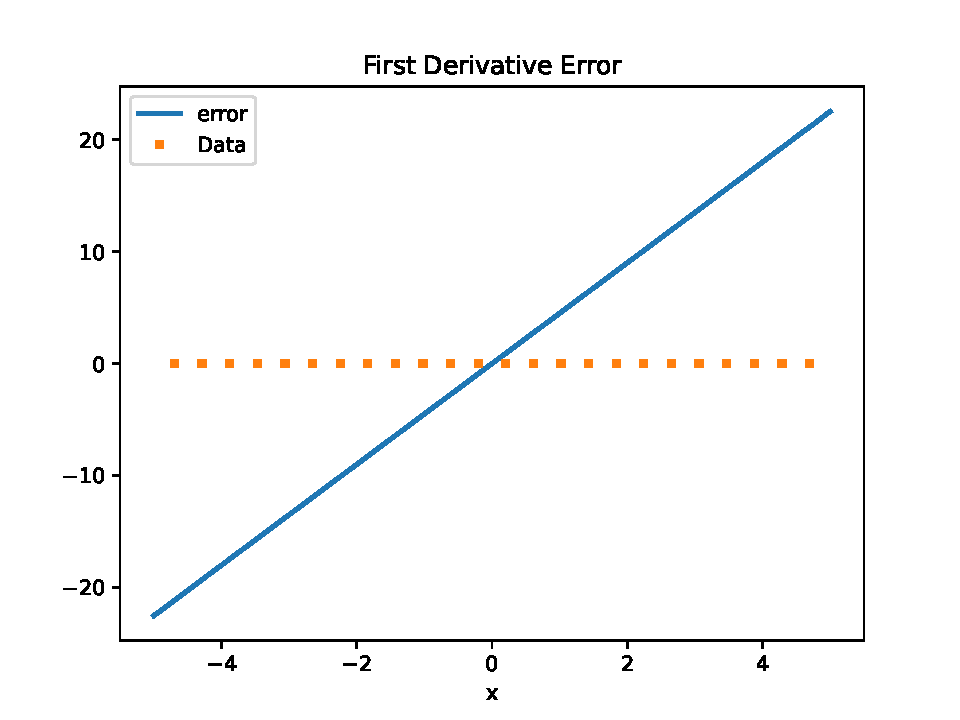
\includegraphics[width=.6\textwidth]{Plots/q2a2.pdf}
            \caption{Error between the interpolated values and the exact values for $f'(x)=12x^3-6x$ on 1 000 points in the interval $[-5,5]$.}
            \label{fig:q2a2}
        \end{center}
    \end{figure}

    \begin{figure}[H]
        \begin{center}
            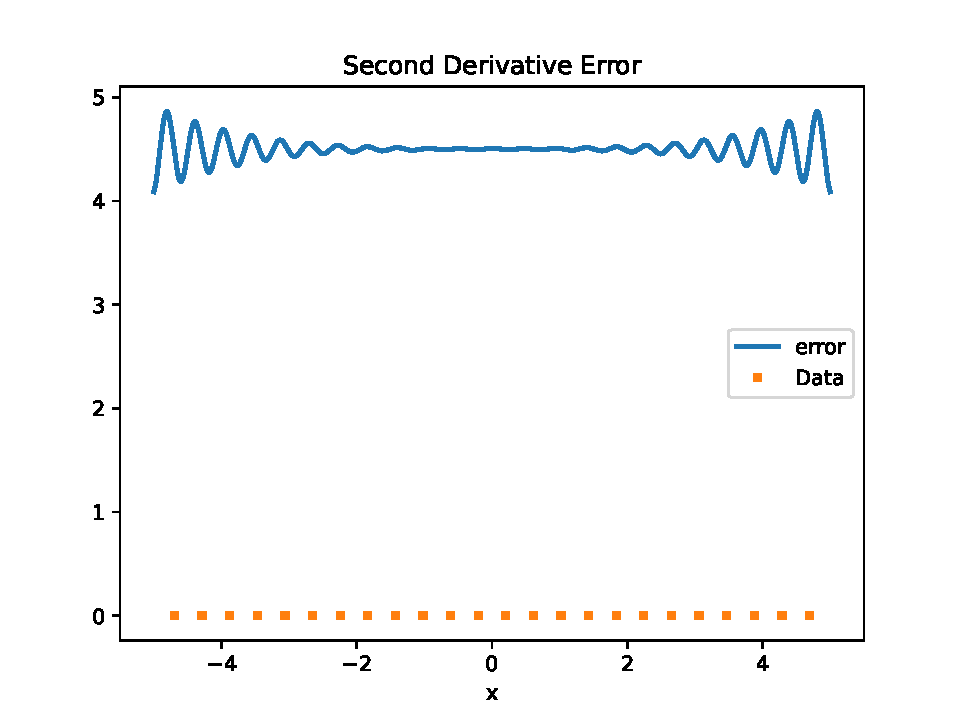
\includegraphics[width=.6\textwidth]{Plots/q2a3.pdf}
            \caption{Error between the interpolated values and the exact values for $f''(x)=36x^2-6$ on 1 000 points in the interval $[-5,5]$.}
            \label{fig:q2a3}
        \end{center}
    \end{figure}

    \textbf{BONUS}\\
    We also considered what effect the parameters, $h$ and $N$, have on the overall error of the interpolation. To do this, we considered $h\in[0.3,1.5]$ and $N\in[15,45]$ and evaluated the overall error as the sum over all interpolation points of the absolute value of the difference between interpolated values and exact values. We did this only for the function evaluation, not any of its derivatives. \Cref{fig:q2b} contains the resulting contour plot.

    \begin{figure}[h]
        \begin{center}
            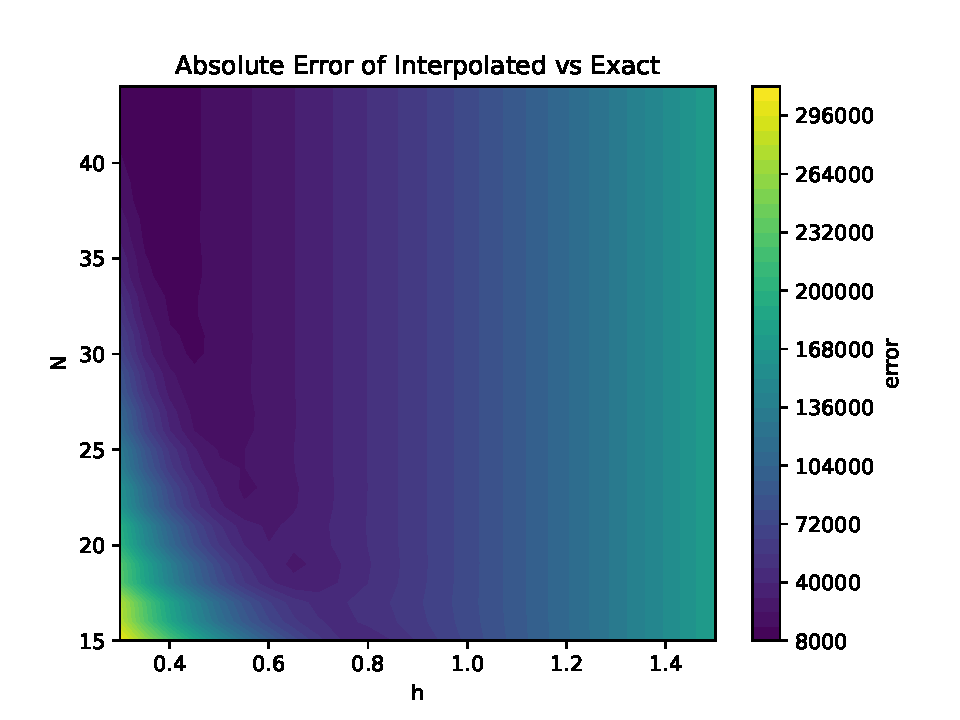
\includegraphics[width=.6\textwidth]{Plots/q2b.pdf}
            \caption{Contour plot of the overall error of SPI for the interpolation of the function $f(x)=3x^4-3x^2$. 1 000 points were interpolated in the interval $[-5,5]$. Overall error was calculated as the sum over all interpolation points of the absolute value of the difference between interpolated values and exact values.}
            \label{fig:q2b}
        \end{center}
    \end{figure}
    
    \item The yield of $\pi^-$ mesons in a hadronic fireball of given temperature $T=\beta^{-1}$, volume $V$, chemical potential $\mu$, and energy $E$ is given by
    \begin{equation}
        N=\frac{V}{2\pi^2}\int_0^\infty dp p^2 \frac{e^{-\beta(E-\mu)}}{1-e^{-\beta(E-\mu)}}
        \label{eqn:pionYield}
    \end{equation}
    Assuming that $p$ is large, we can approximate the energy by $E=\sqrt{p^2+m^2}\approx p$. Then defining $t=\beta p$, so $dt=\beta dp$, we can see
    \begin{align*}
        N&=\frac{V}{2\pi^2}\int_0^\infty dp p^2 \frac{e^{-\beta(p-\mu)}}{1-e^{-\beta(-\mu)}}\\
        &=\frac{V}{2\pi^2}\int_0^\infty \frac{dt}{\beta} \frac{t^2}{\beta^2} e^{-t} \frac{e^{\beta \mu}}{1-e^{\beta\mu}e^{-t}}\\
        &=\frac{Ve^{\beta \mu}}{2\pi^2 \beta^3} \int_0^\infty dt e^{-t} \frac{t^2}{1-e^{\beta\mu}e^{-t}}
    \end{align*}
    Defining $q(t)=\frac{t^2}{1-e^{\beta\mu}e^{-t}}$ we were then able to use Gauss-Laguerre quadrature to find the value of this integral for a given $\mu$. From there, we could use root finding, in our case Regula Falsi, to find the value of $\mu$ for which the yield $N=320$. \\
    
    Some oddities are worth discussing before we present the results: Choosing a number of roots at which to evaluate $q(t)$ when performing the Gauss-Laguerre integration was tricky, as the integrand is not a polynomial. In this case, choosing more roots is better as theoretically it requires infinite function evaluations to converge to the exact value. We chose 20 roots as it seemed to be in the range of numbers used in examples seen online.\\
    With 20 roots, plotting $N(\mu)$ with $T=\SI{0.16e9}{\electronvolt}$ and $r=\SI{6}{\femto\metre}=\SI{3.04064e-8}{\per\electronvolt}$, over the interval $\mu\in [\SI{0.1e9}{\electronvolt},\SI{0.3e9}{\electronvolt}]$ we see \cref{fig:q3a}. No how there appear to be discontinuities in the function at seemingly arbitrary points. We believe this has something to do with the approximation $E\approx p$, since mass is not considered, but we are not sure. \\
    What this affects in relation to finding $\mu$ such that $N=320$, is that the function crosses $N=320$ twice in this interval, so there is no well-defined place to consider this function. To get around this, we assumed that the first discontinuity artificially raised the value of $N$ before it, to above 320, so we should not consider that region. Thus we considered the interval $\mu\in [\SI{0.2e9}{\electronvolt}, \SI{0.25e9}{\electronvolt}]$ when looking for the root, as it seems to be reasonable in that range.\\
    
    Using Regula Falsi, we found the root, $N=320$, to be at $\mu=\SI{0.228784e9}{\electronvolt}$. This is shown in \cref{fig:q3b}.

    \begin{figure}[h]
        \begin{center}
            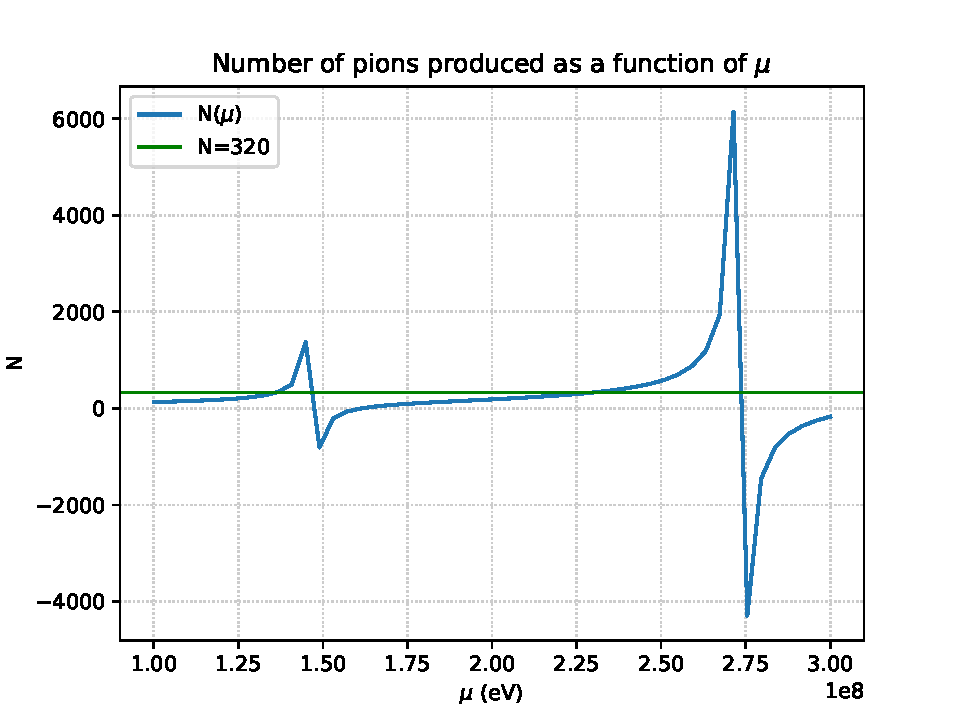
\includegraphics[width=.6\textwidth]{Plots/q3a.pdf}
            \caption{Plot of the number of pions produced, using Gauss-Laguerre quadrature, with $T=\SI{0.16e9}{\electronvolt}$ and $r=\SI{6}{\femto\metre}=\SI{3.04064e-8}{\per\electronvolt}$, over the interval $\mu\in [\SI{0.1e9}{\electronvolt},\SI{0.3e9}{\electronvolt}]$. Shown is the value $N=320$. Note the two discontinuities as well as the function crossing $N=320$ twice.}
            \label{fig:q3a}
        \end{center}
    \end{figure}

    \begin{figure}[h]
        \begin{center}
            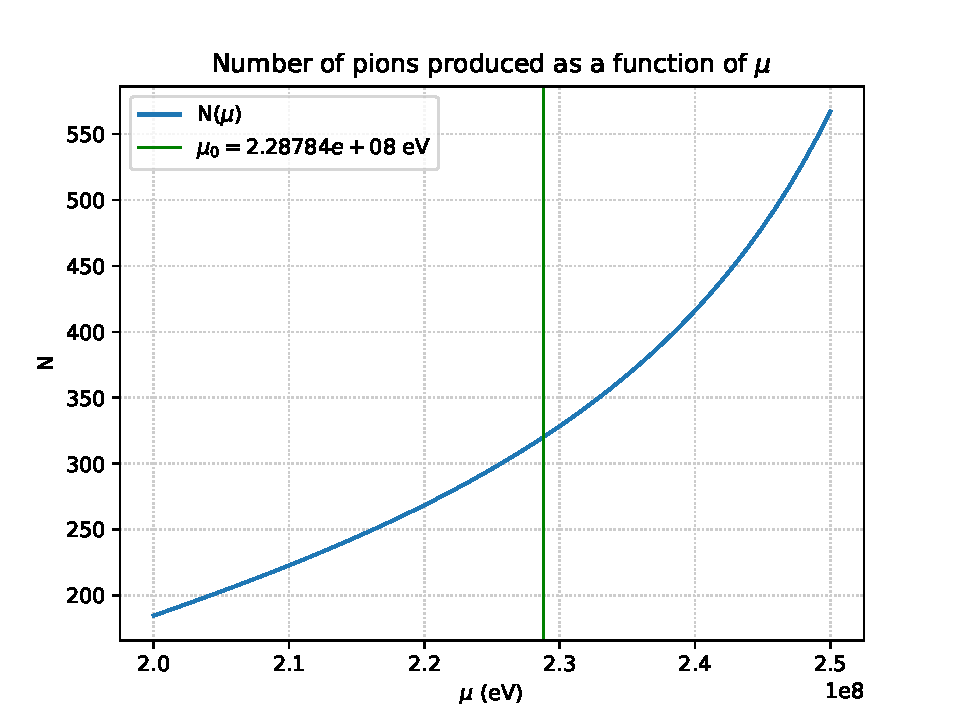
\includegraphics[width=.6\textwidth]{Plots/q3b.pdf}
            \caption{Plot of the number of pions produced, using Gauss-Laguerre quadrature, with $T=\SI{0.16e9}{\electronvolt}$ and $r=\SI{6}{\femto\metre}=\SI{3.04064e-8}{\per\electronvolt}$, over the interval $\mu\in [\SI{0.2e9}{\electronvolt},\SI{0.25e9}{\electronvolt}]$. Shown is the point at which $N(\mu)=320$, found using the Regula Falsi root-finding method.}
            \label{fig:q3b}
        \end{center}
    \end{figure}
    
    

\end{enumerate}

\end{document}